\documentclass[conference]{IEEEtran}
\IEEEoverridecommandlockouts
% The preceding line is only needed to identify funding in the first footnote. If that is unneeded, please comment it out.
\usepackage{cite}
\usepackage[portuges,brazil,english]{babel}
\usepackage{amsmath,amssymb,amsfonts}
\usepackage{algorithmic}
\usepackage{graphicx}
\usepackage{textcomp}
\usepackage{float}
\def\BibTeX{{\rm B\kern-.05em{\sc i\kern-.025em b}\kern-.08em
    T\kern-.1667em\lower.7ex\hbox{E}\kern-.125emX}}
\begin{document}

\title{Predicting Diamonds Price: A Linear Regression Assigment}

\author{\IEEEauthorblockN{Carolina F. Cuba}
\IEEEauthorblockA{
226004 \\
carolinacuba23@gmail.com}
\and
\IEEEauthorblockN{Leonardo de Melo João}
\IEEEauthorblockA{
228118 \\
l228118@g.unicamp.br}}

\maketitle

\section{Introduction}

	Within the field of Machine Learning there are three main categories in which an algorithm can be classified: Supervised Learning Based, Unsupervised Learning Based and Enhancement Learning Based. Supervised systems are developed over a data base that has been already labeled, therefore, we have a previously knowledge of the expected predictions that our model has to return. Supervised learning is typically done in the context of solving both classification and regression problems.
While classification maps an input to a label, regression focus on finding a model that better describes the relationship between the input and output continuous value.\par

	Simple Linear Regression seeks to perform a predictive analysis over an input dataset. Its final result is a set of $\theta$ parameters that are used in linear equation(1) that tries to minimize the prediction error, hence the alternative name given to this function: Cost Function.

\begin{equation}
h_\theta(x)= \theta_0 x_0 + \theta_1 x_1 + \theta_2 x_2 + ... + \theta_n x_n
\end{equation}

The cost function is used to define the best values for $\theta$ parameters that are multiplied to each respectively feature contained in the dataset. In order to find those values, a possibility is to use a method called Gradient Descent. That method consist of applying partial derivatives on the cost function along a series of iterations pre-defined by the user. After each iteration, the $\theta$ parameters are updated given the new cost value and multiplied by a $\alpha$ scalar (learning rate).

\begin{equation}
\theta_n := \theta_n - \alpha \frac{1}{m} \sum_{i=1}^{m} (h_\theta(x^(i)) - y(i))x(i)
\end{equation}

The equation (2) must be repeated by a given number of iterations until the cost reaches a convergence value that coincides with the global minimum of the (1) equation. The importance of the learning rate is that it determines the velocity in which the gradient descent will reach the global minimum. The learning rate has to be set to an appropriate value (neither to low or to high). If it is set to a high value, the gradient descent will not reach the minimum because $\alpha$ will bounces back and forth in the function. If the learning rate is set to a value too low, the gradient descent will eventually reach the minimum, however it will maybe take too much time.\par

The main objective of this assignment is to explore alternatives to linear regression algorithm to solve the problem of predicting the price of diamonds from its attributes using the Diamonds Data Set (54.000 samples). In the "\textit{Activities}" section we explain all the procedures utilized to implement linear regression utilizing both batch and stochastic gradient descent. We also implement a solution for this problem using normalized equations. In the "\textit{Experiments}" section we present all experiments realized, we intended to show relation between cost and number of iterations when changing the method of convergence (gradient descent/normalized equation), the gradient descent itself (batch/stochastic) and the value of learning rate. Finally, on "\textit{Conclusion}" section, we describe all are conclusions after the experimentation.\par

\section{Activities}
In this section we describe all the procedures implemented in order to solve the problem of pricing diamonds. Besides implementing linear regression using batch gradient descent, we also implemented a normalize equation solution for the same problem in order to compare the results and the processing time. This also was our motivation to implement a solution based on stochastic gradient descent.\par
Also, in this section we explain all pre-processing techniques used to prepare the data set in order to achieve better results, among then we can mention: Outliers removal and Dummy feature representation.\par

\subsection{Data Preparation}	
    A requirement for any computerized regression technique is that all data needs to be placed in discretized values and, in our case, three columns were presented as classes: cut, color and clarity. Fortunately, the semantic information of the classes was already given in the dataset description. As an example, the feature 'cut' represents the quality of the cut, as said in the previous section, and it's values are classes, varying among 'fair', 'good', 'very good', 'premium', and 'ideal' in its respective order of quality. That information of the quality order was provided by the description of the dataset.
    
    Thanks to that knowledge, it was decided to use a dummy coding for discretizing the values. That means that we keep the number of features by giving each class a different value. These values respect the semantic increase of quality of the class, i.e. 'fair' = 1, 'good' = 2, 'very good' = 3.
    
    Also, five features are used to represent two pieces of information: x, y, z, depth and table. The size of the diamond is represented by x, y, and z while the depth and table represent the correlation among of these dimensions in percentage. Therefore, we combined x,y,z into a new feature called volume with the correlation among them still being expressed on the depth and table features.
    
    The last pre-processing step in preparation was the normalization of the feature values from a range of 0 to 1. This allows all the features to have similar weights on the gradient descent. It is not always a bad idea to have features weighting differently during the fitting of the model, but due to our team's lack of specific knowledge about diamonds, a less knowledge-driven approach was taken.
    
    With the data prepared for our method, in order to test our model, we started by shuffling our dataset and reserving 15\% of it for future testing, using the remaining 85\% for training. This testing set was put aside until the final results so we wouldn't be biased when presenting our final model. Right after, the training dataset was divided again, with 20\% of it being picked for validation and the remaining 80\% used for the fitness of the model.
    
    After some analysis of the dataset, it was clear that some samples had inconsistent data. There were, for instance, diamonds with volume equal to zero. In that scenario, we used the difference between the mean and the standard deviation of the volume, depth and table columns to remove some of the outliers.
    
\subsection{Implementation}
	As said on previous sessions, this assignment focus on the implementation of three variations of linear regression algorithm to solve the problem of pricing diamonds.\par
    The first implementation was the batch gradient descent. This variation is know for compute the gradient using the whole data base in each iteration. In this case, the algorithm moves almost directly towards an optimum solution. Batch gradient descend really works good on linear regression, were we have convex functions and the global minimum is ensured.\par
    Secondly, we have implemented the stochastic version of gradient descend (SGD) which updates the $\theta$ parameters using a single sample each time. SGD works better on functions that have multiple local minima, because each new iteration tends to remove the model from a local minima to a better one. Besides, another advantage of SGD is that this variation is relatively faster than the batch gradient descent in large data sets.\par
    Finally, we also implemented a normally equation alternative solution this problem. This algorithm does not perform a gradient descend on a function since it directly finds the right values to the $\theta$ parameters using an equation (3) based on linear algebra theory, therefore there is not need of finding the right value of $\alpha$ and there is not need to use a series of iterations.\par

\begin{equation}
\theta = (X^T X)^{-1} X^T y
\end{equation}

This approach, however, only works for linear regression problems, where the model is represented by a convex function. Moreover, this approach can be used for too large data sets because it consumes a lot of RAM memory and its complexity is of O\((n^3)\) .\par

\section{Tests and Experiments}
 	All the experiments presented in this section are easily reproduced by running the python notebook file delivered with this report. The code can also be accessed at Carolina Cuba's github (https://github.com/CarolCuba/ML-Project01). It should be noted that the valued found probably won't be the same due to the sampling part of the data preparation being at random.
	
	Everytime a new test was executed, the result was compared to the normal distribution linear regression as a way to validate if the implemented gradient descent was converging to the expected error, because that equation always finds the global minima in a convex error distribution. 
	
	This equation finds the parameters $\theta$ simply by computing matrices multiplication. To validate the implementation of this equation, we compared it's results on a dummy dataset with Scikit Learn's Linear Model function, which according to the documentation performs the same function.
	
	Also, for accuracy and timing performance tests, the implemented methods were compared to scikit learn's Linear Model SGD\_Classifier, a commonly used python library for machine learning.
	
\subsection{Effects of Data Preparation}
	
    The first experiments with the gradient descent were executed before any data scaling. The algorithm used was the final version of the Batch Gradient Descent without regularization. In that scenario, because of the distance between the feature values, the parameters found were too small to be represented in the float variables in python, causing it to overflow printing the error "overflow encountered in reduce". Because of that error, the gradient descent could never find the minima. Although, the normal equation found the minima with a 1286.71 random mean square error (RMSE). With the learning rate of $1x10^{-5}$ and 10000 iterations, the variable didn't overflow although the rmse was as high as 2015.086.
    
    With the normalized data, the same algorithm could be executed by more iterations and with a higher valued learning rate and the parameters could actually converge to the desired numbers. In this step, we ran a series of tests changing the values of the learning rate ($\alpha$) and the number of iterations. These tests will be detailed in the next subsection, in Table 1.
    
    All the experiments with gradient descent were supported by a chart that shows how the cost (at the y-axis) changes by the number of iterations (at the x-axis). The expected curve is one similar to Figure 1a, which was created by executing the batch gradient descent on the final prepared dataset. 
    
    During a later step of the project, when testing the Stochastic Gradient Descent the $cost x iterations$ plot presented an unexpected curve, as shown in Figure 1b. Even though the stochastic gradient descent has a noisier curve compared to the smooth batch generated curve, the steep sudden changes gave us the insight to look for outliers.
	
	\begin{figure*}[!h]
      \centering
      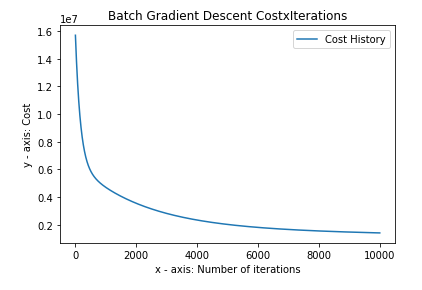
\includegraphics[width=0.48\textwidth]{images/smooth-gd-curve.png}
      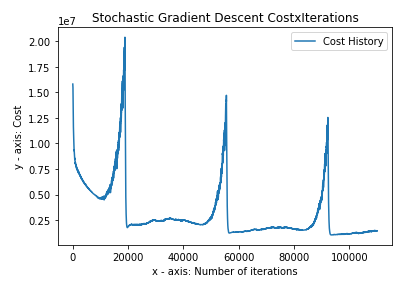
\includegraphics[width=0.48\textwidth]{images/steep-curves-in-stochastic-gd.png}
      \caption{Smooth curve and Stochastic unexpect curve due to unshuffling and outliers, respectively}
      \label{fig1}
  \end{figure*}
	
    The outlier removal technique was based on the mean and standard deviation. Each sample's features should have its values falling in between the product of the feature's mean and its standard deviation. The described method was good enough to remove clear outliers (diamonds with a volume value equal to zero, for instance). Although, the stochastic curve presented the same behavior.
    
    After close analysis, the behavior was due to the data being ordered in an ascending order which was causing the unexpected behavior. After a simple shuffling of the data frame, the stochastically generated graphic was quite similar to the batch curve, as shown in Figure 2.
	
  \begin{figure}[!h]
      \centering
      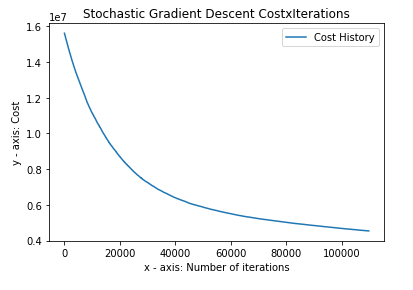
\includegraphics[width=1\columnwidth]{images/smoother-curves-in-stochastic-gd.png}
      \caption{Smooth stochastic gradient descent curve}
      \label{fig2}
  \end{figure}
	
\section{Time and Accuracy Performance Tests}

	The time and accuracy performance tests were held in the validation slice of the dataset while comparing different learning rates in both methods (batch and stochastic GD). Afterwards, the better fitted model was used in the actual test set to check the final (and more realistic) accuracy.
	
	Table 1 shows the number of iterations and time it took for both algorithms to reach a desired error variation between iterations of $\epsilon$  = $1x10^{-5}$ or a max number of iterations equal to 5 times the number of samples in the training dataset.
	
	  \begin{table}[h!]
    \begin{center}
      \caption{Performance tests for different learning rates}
      \label{table:table1}
      \begin{tabular}{l|c|c|c|c}
        Method & Learning Rate & Iterations & Time(s) & RMSE\\
        \hline
        Batch & 0.001 & 51523 & 289.135 & 2502.948 \\
        Stochastic & 0,001 & 183190 & 586,639 & 2494.971 \\
        Batch & 0.005 & 40892 & 223.085 & 1690.667 \\
        Stochastic & 0.005 & 183190 & 578.814 & 1678.273 \\
        Batch & 0.01 & 31954 & 181.066 & 1482.209 \\
        Stochastic & 0.01 & 183190 & 620.516 & 1470.200 \\
        Batch & 0.05 & 26753 & 155.024 & 1280.599 \\
        Stochastic & 0.05 & 183190 & 642.264 & 1502,134 \\
        Batch & 0.1 & 24872 & 143.273 & 1265.195 \\
        Stochastic & 0.1 & 183190 & 651.987 & 1912,245 \\
        Batch & 0.5 & 22077 & 124.462 & 1260.281 \\
        Stochastic & 0.5 & 183190 & 669.826 & 2566.960 \\
    \end{tabular}
  \end{center}
\end{table}	
	
	Analysing the table, the Batch Gradient Descent(BGD) performed better in this dataset, with  both the number of iterations and Random Mean Square Error (RMSE) decreasing on the increase of the learning rate.
	
	On the other hand, the Stochastic Gradient Descent (SGD) performed well in accuracy until a learning rate of 0.001 but couldn't converge to a minima with values greater than this. In order to check this behavior a chart was plotted to show how the cost was changing over time. The result (Figure 3) chart shows that the learning rate was causing the SGD to miss the local minima constantly, never converging to the desired value.
	
	  \begin{figure}[!h]
      \centering
      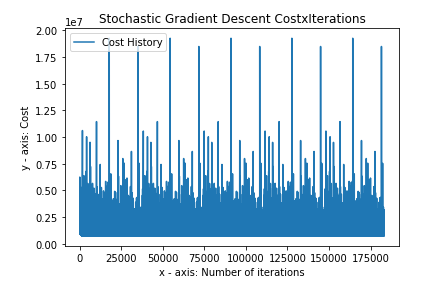
\includegraphics[width=1\columnwidth]{images/sgd_high_learning_rate.png}
      \caption{High learning rate SGD missing the minima}
      \label{fig3}
  \end{figure}
	
	Still analysing the table, the fixed number of iterations in the SGD is due to a lack of convergence to the desired error variation described in a few paragraphs above. Because the parameters ($\theta_i$) are updated after each sample, the error between the updates is higher, causing the unwanted waiting time.
	
	Based on these results, the best model in both time nad RMSE was the BGD with a learning rate of 0.5 and it was the one selected for running on the test set.

	In order to compare the test results, an execution of the Normal Equation Regression algorithm developed in this work and the Scikit SGD were also used to calculte the error. The  implemented BGD got an RMSE of 1210.178 and it took 120.651 seconds to run while the normal equation got a 1892.386 RMSE and took 0.005 seconds to run. In it's turn, the Scikit Learn SGD got an RMSE of 4723.090 and it took 49 seconds to run, using the same cost function, epsulon, learning rate and maximum number of iterations. These results are easily visualized on Table 2.
	
	The reason why the scikit method converged so poorly is because of the relation between learning rate and max number of iteraions (as seen in Table one's comparison between BGD and SGD). In order for it to converge, the learning rate should be quite smaller and the max number of iterations should be higher.
	
	The difference between the Normal Equation values compared to the others was unexpected, since this algorithm should find the optimum minima. Although, when tested on the training set, it performed better than all other algorithms. This means that the normal equation was overfitting the training set, even though the model is a simple line.
	
  \begin{table}[h!]
    \begin{center}
      \caption{Performance tests for different models}
      \label{table:table2}
      \begin{tabular}[10pt]{c|c|c|c}
        Method & Learning Rate & Time(s) & RMSE\\
        \hline
        Implemented BGD & 0.5 & 120.651 & 1210.948 \\
        Sckiti SGD& 0.5 & -69.49554800987244 & 4723.090 \\
        Normal Equation & - & 0.005 & 1193.825 \\
    \end{tabular}
  \end{center}
\end{table}
	

\section{Conclusion}



\end{document}
